\lab{Conservation Laws and Heat Flow}{Heat Flow}
\label{lab:HeatFlow}
\labdependencies{FiniteDifferenceMethod}

Many physical phenomena have a conservation law associated with them.
For instance, matter, energy, and momentum are all conserved quantities.
The \textit{fundamental conservation law} states that the rate of change of the total quantity in the system is equal to the rate that the quantity enters the system plus the rate at which the quantity is produced by sources inside the system.
While this is a \textit{global} property, we can use it to obtain a \textit{local} differential equation that the concentration of the quantity must obey everywhere in the system.
Because of this, conservation laws are very important in modeling a wide variety of phenomena.

\section*{Derivation of the Conservation equation in multiple dimensions}
Suppose $\Omega$ is a region in $\mathbb{R}^n$, and $V \subset \Omega$ is bounded with a reasonably well-behaved boundary $\partial V$.
Let $u(\vec{x},t)$ represent the density (concentration) of some quantity throughout $\Omega$.
Let $\vec{n}(x)$ represent the normal direction to $V$ at $x \in \partial V$, and let $\vec{J}(\vec{x},t)$ be the flux vector for the quantity, so that $\vec{J}(\vec{x},t) \cdot \vec{n}(x) \, dA$ represents the rate at which the quantity leaves $V$ by crossing a boundary element with area $dA$.
Note that the total amount of the quantity in $V$ is
\[ \int_V u(\vec{x},t)\, dt,\]
and the rate at which the quantity enters $V$ is
\[-\int_{\partial V} \vec{J}(\vec{x},t) \cdot \vec{n}(x) \, dA.\]

We let the source term be given by $g(\vec{x},t,u)$; we may interpret this to mean that the rate at which the quantity is produced in $V$ is
\[\int_V g(\vec{x},t,u)\, dt.\]
Then the integral form of the conservation law for $u$ is expressed as
\[\frac{d}{dt} \int_V u(\vec{x},t) \, d\vec{x} = -\int_{\partial V} \vec{J}\cdot \vec{n}\, dA + \int_V g(\vec{x},t,u)\, d\vec{x}.\]

If $u$ and $J$ are sufficiently smooth functions, then we have
\[ \frac{d}{dt} \int_V u\, d\vec{x} = \int_V u_t \, d\vec{x},\]
and
\[ \int_{\partial V} \vec{J}\cdot \vec{n}\, dA = \int_V \nabla \cdot \vec{J}\, d\vec{x} .\]
Putting these together yields
\[
\int_Vu(\vec x,t)\,d\vec x = \int_V\left(
-\nabla\cdot \vec{J} + g(\vec{x},t,u)
\right)\,d\vec x
\]
Since this holds for all nice subsets $V \subset \Omega$ with $V$ arbitrarily small, the integrands must be equal everywhere, and we obtain the differential form of the conservation law for $u$:
\[ u_t + \nabla \cdot \vec{J} = g(\vec{x},t,u) ,\]
where $\nabla$ is the gradient operator and $\nabla \cdot \vec{J} = \frac{\partial J_1}{\partial x_1} + \dots + \frac{\partial J_n}{\partial x_n}$

\section*{Constitutive Relations}
So far, our conservation law consists of 2 unknowns ($u$ and $J$) but only 1 equation.
To this equation we need to add other equations, called \textit{constitutive relations}, which are used to fully determine the system.

For example, suppose we wish to model the flow of heat.
Since heat flows from warmer regions to colder regions, and the rate of heat flow depends on the difference in temperature between regions, we usually assume that the flux vector $\vec{J}$ is given by
\[\vec{J}(x,t) = -\nu \nabla u(x,t),\]
where $\nu$ is called the diffusion constant and $\nabla u(x,t) = \left[ \partial_{x_1}u, \dots, \partial_{x_n}u\right]^T$.
This constitutive relation is called Fick's law, and is the basic model for any diffusive process.
Substituting into the conservation law we obtain
\[u_t -\nu \Delta u(x,t) = g(\vec{x},t,u)\]
where $\Delta$ is the Laplacian operator:
\[\Delta u(x,t) = \frac{\partial ^2 u}{\partial x_1^2}+\dots+ \frac{\partial ^2 u}{\partial x_n^2}.\]
The function $g$ represents heat sources and sinks within the region.

\section*{Numerically modeling heat flow}
Consider the heat flow equation in one dimension together with an appropriate initial condition \(u(x,0)=f(x)\), homogeneous Dirichlet boundary conditions, and \(g(x,t,u)=0\):
\begin{align*}
	&{ } u_t = \nu u_{xx}, \quad x \in [a,b],\quad t \in [0,T], \\
	&{ } u(a,t) = 0,\quad u(b,t) = 0,\\
	&{ } u(x,0) = f(x).
\end{align*}
We will create an approximation $U^m_j$ to $u(x_j,t_m)$ on the grid $x_j = a +  hj$, $t_m = km$, where $h$ and $k$ are small changes in $x$ and $t$ respectively and $j$ and $m$ are indices; so, \(U_j^m\) denotes the approximate value of $u$ at the $j$-th grid point and the $m$-th time step.
%Note that the index $j$ ranges over different spacial grid points and the index $m$ ranges over different time steps.

\begin{comment}
A common method for modeling ordinary and partial differential equations is the finite difference method, so-named because equations containing derivatives are replaced with equations containing difference schemes.
These difference schemes can often be found using Taylor's theorem.
For example, the equation
\begin{align*}
	u(x,t_m + k) = u(x,t_m) + u_t(x,t_m)k + \mathcal{O}(k^2)
\end{align*}
yields a first-order forward difference approximation to $u_t(x,t_m)$, namely,
\begin{align*}
	u_t(x,t_m ) = \frac{u(x,t_m+k) - u(x,t_m)}{k} + \mathcal{O}(k).
\end{align*}
Similarly, by adding the equations
\begin{align*}
	u(x_j+h,t) &= u(x_j,t) + u_x(x_j,t)h + u_{xx}(x_j,t)\frac{h^2}{2} + u_{xxx}(x_j,t)h^3 + \mathcal{O}(h^4),\\
	u(x_j-h,t) &= u(x_j,t) + u_x(x_j,t)(-h) + u_{xx}(x_j,t)\frac{(-h)^2}{2} + u_{xxx}(x_j,t)(-h)^3 + \mathcal{O}(h^4),
\end{align*}
we obtain a second-order centered difference approximation to $u_{xx}(x_j,t)$:
\begin{align*}
	u_{xx}(x_j,t_m) &= \frac{u(x_j + h,t_m )-2 u(x_j,t_m)- u(x_j - h,t_m)}{h^2} + \mathcal{O}(h^2).
\end{align*}
\end{comment}

As before, we will use the finite difference method to create this approximation.
Recall that by using Taylor's theorem, we have the first-order forward difference approximation
\begin{align*}
	u_t(x,t) = \frac{u(x,t+k) - u(x,t)}{k} + \mathcal{O}(k).
\end{align*}
and the second-order centered difference approximation
\begin{align*}
	u_{xx}(x_j,t_m) &= \frac{u(x_j + h,t_m )-2 u(x_j,t_m)- u(x_j - h,t_m)}{h^2} + \mathcal{O}(h^2).
\end{align*}

\begin{figure}
\centering
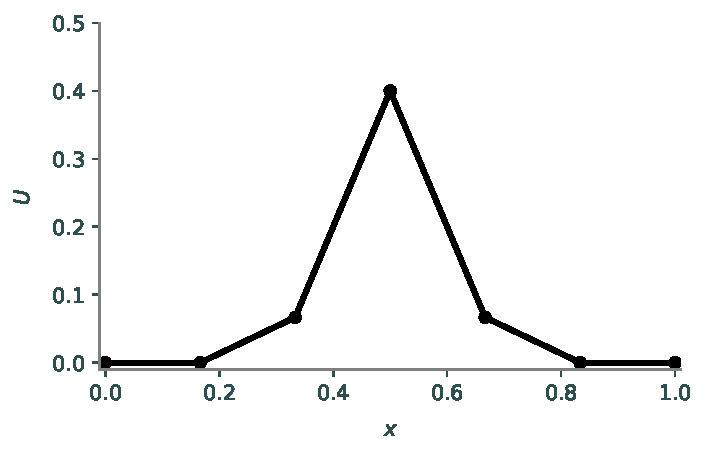
\includegraphics[width=\textwidth]{figures/heatexercise1a.pdf}
\caption{The graph of $U^{0}$, the approximation to the solution $u(x,t=0)$ for Problem \ref{prob:heat_exercise1}.}
\label{fig:heatexercise1a}
\end{figure}

\noindent
Applying these difference approximations give us the $\mathcal{O}(h^2 + k)$ explicit method
\begin{align}
	\begin{split}
	\frac{U_{j}^{m+1} - U_{j}^{m}}{k} &= \nu \frac{U_{j+1}^{m}- 2U_{j}^{m} + U_{j-1}^{m} }{h^2} ,\\
	U_{j}^{m+1} &= U_{j}^{m} + \frac{\nu k}{h^2} (U_{j+1}^{m}- 2U_{j}^{m} + U_{j-1}^{m} ).
	\end{split}\label{eqn:firstorder_explicit}
\end{align}
This method can be written in matrix form as
\[U^{m+1} = A U^m,\]
where $A$ is the $(n-1) \times (n-1)$ tridiagonal matrix given by
\[A = \left[\begin{array}{cccccc}1 & 0 & & & \\ \lambda & 1-2\lambda & \lambda & & \\ & \ddots & \ddots & \ddots & \\ & & \lambda & 1-2\lambda & \lambda \\  &  &  & 0 & 1\end{array}\right],\]
where $\lambda = \nu k/h^2$, $n$ is the number of spatial subintervals, and $U^m$ represents the approximation at time $t_m$.
We can initialize this method using the initial condition given in our problem, which tells us that $U_{j}^{0} = f(x_j)$.

\begin{figure}
\centering
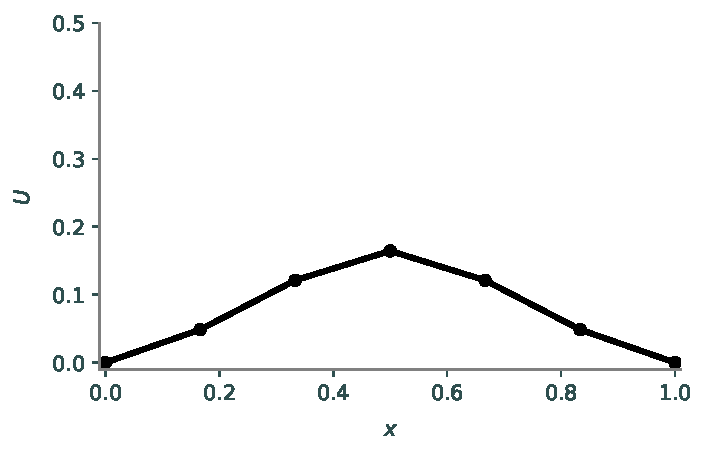
\includegraphics[width=\textwidth]{figures/heatexercise1b.pdf}
\caption{The graph of $U^{4}$, the approximation to the solution $u(x,t=0.4)$ for Problem \ref{prob:heat_exercise1}.}
\label{fig:heatexercise1b}
\end{figure}

\begin{info}
Note that the matrix representing the finite difference scheme is very \emph{sparse}, which is typical of finite difference schemes.
While represeting finite difference schemes with matrices can be an effective method, especially for implicit schemes, it is very important that a sparse matrix format is used.
Otherwise, performance will be dramaticaly negatively impacted.
In Python, since looping is slow, the best alternative is to vectorize the difference scheme.
This approach can in fact be even better than using matrices for explicit schemes, such as the one we are using here, as it avoids needing to store the matrix in memory.
\end{info}

To account for our constant boundary conditions using this differencing scheme, simply set the boundary points to the appropriate values in the initial conditions, then avoid modifying them as you update for each time step.
Note that the first and last rows of the matrix representation of the differencing scheme are the same as the first and last rows of the identity matrix.
This has the effect of keeping the boundary points the same as in the previous step, and thus the same as in the initial condition.

\begin{problem}
\label{prob:heat_exercise1}
Consider the initial/boundary value problem
\begin{align}
	\begin{split}
	&{ } u_t = 0.05 u_{xx}, \quad x \in [0,1], \quad t \in [0,1]\\
	&{ } u(0,t) = 0,\quad u(1,t) = 0,\\
	&{ } u(x,0) = 2\max\{0.2 - |x-0.5|,0\}.
	\end{split}
\end{align}
Approximate the solution $u(x,t)$ by taking 6 subintervals in the $x$ dimension and 10 subintervals in time.
Plot the solution at the times \(t=0, t=0.4,\) and \(t=1\).
The graphs for $U^0$ and $U^{4}$ are given in Figures \ref{fig:heatexercise1a} and \ref{fig:heatexercise1b}.
\end{problem}

\begin{comment}
For the next problem, we need to show how Matplotlib can be used to create a 2D animation.
The following is a simple working example that animates a sine wave.

\begin{lstlisting}
import numpy as np
from matplotlib import animation, pyplot as plt

def sine_animation(res=100):
    # Make the x and y data.
    x = np.linspace(-1, 1, res+1)[:-1]
    y = np.sin(np.pi * x)
    # Initialize a matplotlib figure.
    f = plt.figure()
    # Set the x and y axes by constructing an axes object.
    plt.axes(xlim=(-1,1), ylim=(-1,1))
    # Plot an empty line to use in the animation.
    # Notice that we are unpacking a tuple of length 1.
    line, = plt.plot([], [])
    # Define an animation function that will update the line to
    # reflect the desired data for the i'th frame.
    def animate(i):
        # Set the data for updated version of the line.
        line.set_data(x, np.roll(y, i))
        # Notice that this returns a tuple of length 1.
        return line,
    # Create the animation object.
    # 'frames' is the number of frames before the animation should repeat.
    # 'interval' is the amount of time to wait before updating the plot.
    # Be sure to assign the animation a name so that Python does not
    # immediately garbage collect (delete) the object.
    a = animation.FuncAnimation(f, animate, frames=y.size, interval=20)
    # Show the animation.
    plt.show()

# Run the animation function we just defined.
sine_animation()
\end{lstlisting}
\end{comment}

\begin{problem}
\label{prob:heat_exercise2}
Solve the initial/boundary value problem
\begin{align}
	\begin{split}
	&{ } u_t = u_{xx}, \quad x \in [-12,12],\quad t \in [0,1], \\
	&{ } u(-12,t) = 0,\quad u(12,t) = 0,\\
	&{ } u(x,0) = \max\{1 - x^2,0\}
	\end{split}
\end{align}
using the first order explicit method \ref{eqn:firstorder_explicit}.
Use 140 subintervals in the $x$ dimension and 70 subintervals in time.
The initial and final states are shown in Figure \ref{fig:heatexercise2}.
Animate your results.

Explicit methods usually have a stability condition, called a CFL condition (for Courant-Friedrichs-Lewy).
For method \ref{eqn:firstorder_explicit} the CFL condition that must be satisfied is that
\[\lambda=\frac{\nu k}{h^2} \leq \frac{1}{2}.\]
Repeat your computations using 140 subintervals in the $x$ dimension and 66 subintervals in time. Animate the results.
For these values, the CFL condition is broken; you should be able to clearly see the result of this instability in the approximation $U^{66}$.
\end{problem}

\begin{figure}
\centering
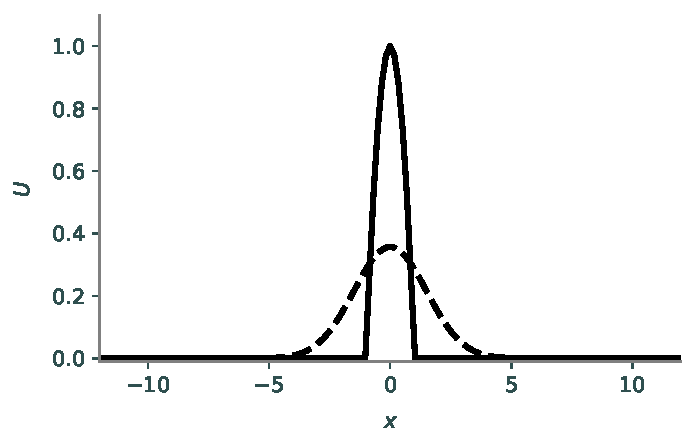
\includegraphics[width=\textwidth]{figures/heatexercise2.pdf}
\caption{The initial and final states for equation Problem \ref{prob:heat_exercise2}.}
\label{fig:heatexercise2}
\end{figure}

Implicit methods often have better stability properties than explicit methods.
The Crank-Nicolson method, for example, is unconditionally stable and has order $\mathcal{O}(h^2 + k^2)$.
To derive the Crank-Nicolson method, we use the following approximations:
\begin{align*}
	u_t(x_j,t_{m+1/2}) &= \frac{u(x_j,t_{m+1}) - u(x_j,t_m)}{k} + \mathcal{O}(k^2), \\
	u_{xx}(x_j,t_{m+1/2}) &= \frac{u_{xx}(x_j,t_{m+1}) + u_{xx}(x_j,t_m)}{2} + \mathcal{O}(k^2).
\end{align*}
The first equation is a finite difference approximation for \(u_t\), and the second is a midpoint approximation applied to \(u_{xx}\). 
These approximations give the relation
\begin{align}
	\begin{split}
	\frac{U^{m+1}_j - U^m_j}{k} &= \frac{1}{2}\left( \frac{U^m_{j+1} - 2U^m_{j} + U^m_{j-1}}{h^2} + \frac{U^{m+1}_{j+1} - 2U^{m+1}_{j} + U^{m+1}_{j-1}}{h^2}  \right) ,\\
	U^{m+1}_j  &= U^m_j + \frac{k}{2h^2} \left( U^m_{j+1} - 2U^m_{j} + U^m_{j-1} + U^{m+1}_{j+1} - 2U^{m+1}_{j} + U^{m+1}_{j-1}   \right).
\end{split}
\end{align}
This method can be written in matrix form as
\[BU^{m+1} = A U^m,\]
where $A$ and $B$ are tridiagonal matrices given by
\begin{align*}
B &= \left[\begin{array}{cccccc}1 & 0 &  &  &  \\ -\lambda & 1+2\lambda &  -\lambda & &  \\ &  \ddots &   \ddots & \ddots \\ & &  -\lambda &  1+2\lambda & -\lambda \\ &  &  & 0 & 1\end{array}\right], \\
A &= \left[\begin{array}{cccccc}1 & 0 &  &  &  \\ \lambda & 1-2\lambda &  \lambda & &  \\ &  \ddots &   \ddots & \ddots \\ & &  \lambda &  1-2\lambda & \lambda \\ &  &  & 0 & 1\end{array}\right],
\end{align*}
where $\lambda = \nu k/(2h^2)$, and $U^m$ represents the approximation at time $t_m$.
Note that here we have defined $\lambda$ differently than we did before!

How do we know if a numerical approximation is reasonable?
One way to determine this is to compute solutions for various step sizes $h$ and see if the solutions are converging to something, which we hope to be the true solution.
To be more specific, suppose our finite difference method is $\mathcal{O}(h^p)$ accurate.
This means that the error $E(h) \approx Ch^p$ for some constant $C$ as $h \to 0$ (that is, for $h>0$ small enough).

So, we will compute the approximation $y_k$ for each stepsize $h_k$, $h_1 > h_2> \ldots>h_q.$
We will think of $y_q$ as the true solution.
Then the error of the approximation for stepsize $h_k, k < q,$ is
\begin{align*}
	E(h_k) &= \max( \abs{ y_k - y_q}) \approx C h_k^p ,\\
	\log(E(h_k)) &= \log(C) + p \log(h_k).
\end{align*}
Thus on a log-log plot of $E(h)$ vs. $h,$ these values should be on a straight line with slope $p$ when $h$ is small enough to start getting convergence.

\begin{figure}
\centering
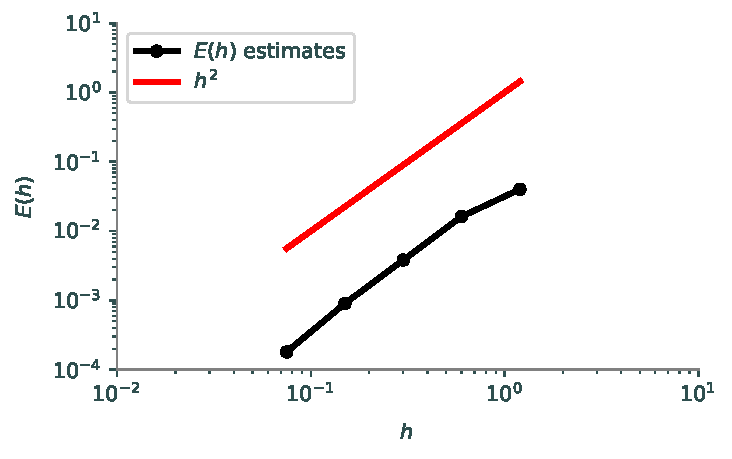
\includegraphics[width=\textwidth]{figures/MaximumError.pdf}
\caption{$E(h)$ represents the (approximate) maximum error in the numerical solution $U$ to Problem \ref{prob:heat_exercise3} at time $t=1$, using a stepsize of $h$.}
\label{fig:heatexercise3}
\end{figure}

\begin{problem}
\label{prob:heat_exercise3}
Using the Crank Nicolson method, numerically approximate the solution $u(x,t)$ of the problem
\begin{align}
	\begin{split}
	&{ } u_t = u_{xx}, \quad x \in [-12,12],\quad t \in [0,1],\\
	&{ } u(-12,t) = 0,\quad u(12,t) = 0,\\
	&{ } u(x,0) = \max\{1 - x^2,0\}.
	\end{split}
\end{align}
Note that this is an implicit linear scheme; hence, the most efficient way to find \(U^{m+1}\) is to create the matrix \(B\) as a sparse matrix and use \li{scipy.sparse.linalg.spsolve}.

Demonstrate that the numerical approximation at $t = 1$ converges.
Do this by computing $U$ at $t=1$ using $20,40,80,160,320$, and $640$ intervals.
Use the same number of steps in both time and space.
Reproduce the loglog plot shown in Figure \ref{fig:heatexercise3}.
The slope of the line there shows the order of convergence.

To measure the error, use the solution with the smallest $h$ (largest number of intervals) as if it were the exact solution, then sample each solution only at the x-values that are represented in the solution with the largest $h$ (smallest number of intervals).
Use the $\infty$-norm on the arrays of values at those points to measure the error.

Notice that, since the Crank-Nicolson method is unconditionally stable, there is no CFL condition, and we can safely use the same number of intervals in time and space.
\end{problem}